\documentclass{scrartcl}
 
\usepackage[utf8]{inputenc}
\usepackage[T1]{fontenc}
\usepackage{lmodern}
\usepackage[pdftex]{graphicx}
\usepackage[ngerman]{babel}
\usepackage{amsmath}
\usepackage{amssymb}
\usepackage{tabularx}
\usepackage{multirow}
\usepackage{amsfonts}
\usepackage{tabto}
\usepackage{mathtools}
\TabPositions{0.1in, 0.4in, 0.6in, 0.8in, 1.0in, 1.2in, 3.4in}

\begin{document}
\begin{LARGE}
Spieltheorie - WiSe 2014/15
\end{LARGE}

\begin{Large}
Übungsblatt 9 - Felix Dosch\\[1.0cm]
\end{Large}

\begin{Large}
Aufgabe 9.1\\[0.0cm]
\end{Large}

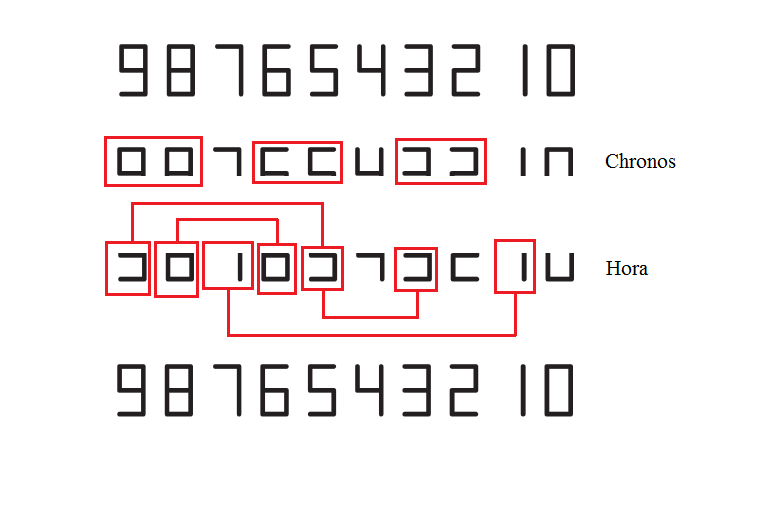
\includegraphics[width=1\textwidth]{times.png}

Wir betrachten die Anzeige der Uhr im Folgenden durch die Ziffern $h_1, h_2, m_1$ und $m_2$,
dabei ist die Anzeige im Format $h_1h_2:m_1m_2$. \\

a) \\

Chronos kann aus der Menge $\{0, ..., 9\}$ die Ziffern 0, 1, 4 und 7 unterscheiden (siehe
Abbildung). Das heißt, für die Stelle $m_2$ kann er diese Ziffern unterscheiden. Ist
$h_1 < 2$, so kann er ebenfalls für $h_2$ diese Ziffern unterscheiden. Ist $h_2$ = 2, so 
kann er dort zwischen 0 und 1 unterscheiden (4 und 7 können nicht vorkommen). \\

Da $h_1$ nur aus der Menge \{0, 1, 2\} sein kann, kann er diese Ziffern alle unterscheiden
(In \{0, ..., 9\} kann er lediglich die 2 nicht von der 3 unterscheiden). \\

Da $m_1$ nur aus der Menge \{0, 1, ..., 5\} sein kann, kann er zusätzlich zu 0, 1 und 4 auch
die 5 unterscheiden (In \{0, ..., 9\} kann er lediglich die 5 nicht von der 6 unterscheiden). \\

Es gibt also folgende Vorgaben für die Zeiten $h_1h_2:m_1m_2$:

\begin{itemize}
\item{$h_1 \in \{0, 1, 2\}$}
\item{$h_2 \in \{0, 1, 4, 7\}$, falls $h_1 < 2$}
\item{$h_2 \in \{0, 1\}$, falls $h_1 = 2$}
\item{$m_1 \in \{0, 1, 4, 5\}$}
\item{$m_2 \in \{0, 1, 7, 7\}$}
\end{itemize}

Als Gesamtzahl möglicher Uhrzeiten, die Chronos genau erkennen kann, ergibt sich damit
$2 \cdot 4 \cdot 4 \cdot 4 + 2 \cdot 4 \cdot 4 = 160.$ Die einzelnen Uhrzeiten lauten: \\

00:00, 00:01, 00:04, 00:07, 00:10, 00:11, 00:14, 00:17, 00:40, 00:41, 00:44, 00:47,
00:50, 00:51, 00:54, 00:57, 01:00, 01:01, 01:04, 01:07, 01:10, 01:11, 01:14, 01:17, 01:40, 
01:41, 01:44, 01:47, 01:50, 01:51, 01:54, 01:57, 04:00, 04:01, 04:04, 04:07, 04:10, 04:11, 
04:14, 04:17, 04:40, 04:41, 04:44, 04:47, 04:50, 04:51, 04:54, 04:57, 07:00, 07:01, 07:04, 
07:07, 07:10, 07:11, 07:14, 07:17, 07:40, 07:41, 07:44, 07:47, 07:50, 07:51, 07:54, 07:57,
10:00, 10:01, 10:04, 10:07, 10:10, 10:11, 10:14, 10:17, 10:40, 10:41, 10:44, 10:47, 10:50, 
10:51, 10:54, 10:57, 11:00, 11:01, 11:04, 11:07, 11:10, 11:11, 11:14, 11:17, 11:40, 11:41, 
11:44, 11:47, 11:50, 11:51, 11:54, 11:57, 14:00, 14:01, 14:04, 14:07, 14:10, 14:11, 14:14, 
14:17, 14:40, 14:41, 14:44, 14:47, 14:50, 14:51, 14:54, 14:57, 17:00, 17:01, 17:04, 17:07, 
17:10, 17:11, 17:14, 17:17, 17:40, 17:41, 17:44, 17:47, 17:50, 17:51, 17:54, 17:57, 20:00, 
20:01, 20:04, 20:07, 20:10, 20:11, 20:14, 20:17, 20:40, 20:41, 20:44, 20:47, 20:50, 20:51,
20:54, 20:57, 21:00, 21:01, 21:04, 21:07, 21:10, 21:11, 21:14, 21:17, 21:40, 21:41, 21:44,
21:47, 21:50, 21:51, 21:54, 21:57 \\

b) Hier nicht ganz so ausführlich wie in a). Hora kann aus der Menge $\{0, ..., 9\}$ die Ziffern
0, 2 und 4 unterscheiden (siehe Abbildung).

\begin{itemize}
\item{$h_1 \in \{0, 1, 2\}^1$}
\item{$h_2 \in \{0, 2, 4\}$, falls $h_1 < 2$}
\item{$h_2 \in \{0, 1, 2, 3\}^{1,2}$, falls $h_1 = 2$}
\item{$m_1 \in \{0, 1, 2, 4\}^1$}
\item{$m_2 \in \{0, 2, 4\}$}
\end{itemize}

$^1$ = kann 1 erkennen, da 7 nicht vorkommt

$^2$ = kann 3 erkennen, da 5 und 9 nicht vorkommen. \\

Gesamtzahl: $2 \cdot 3 \cdot 4 \cdot 3 + 4 \cdot 4 \cdot 3 = 120.$ Die einzelnen Uhrzeiten: \\

00:00, 00:02, 00:04, 00:10, 00:12, 00:14, 00:20, 00:22, 00:24, 00:40, 00:42, 00:44, 02:00,
02:02, 02:04, 02:10, 02:12, 02:14, 02:20, 02:22, 02:24, 02:40, 02:42, 02:44, 04:00, 04:02,
04:04, 04:10, 04:12, 04:14, 04:20, 04:22, 04:24, 04:40, 04:42, 04:44, 10:00, 10:02, 10:04,
10:10, 10:12, 10:14, 10:20, 10:22, 10:24, 10:40, 10:42, 10:44, 12:00, 12:02, 12:04, 12:10,
12:12, 12:14, 12:20, 12:22, 12:24, 12:40, 12:42, 12:44, 14:00, 14:02, 14:04, 14:10, 14:12,
14:14, 14:20, 14:22, 14:24, 14:40, 14:42, 14:44, 20:00, 20:02, 20:04, 20:10, 20:12, 20:14,
20:20, 20:22, 20:24, 20:40, 20:42, 20:44, 21:00, 21:02, 21:04, 21:10, 21:12, 21:14, 21:20,
21:22, 21:24, 21:40, 21:42, 21:44, 22:00, 22:02, 22:04, 22:10, 22:12, 22:14, 22:20, 22:22,
22:24, 22:40, 22:42, 22:44, 23:00, 23:02, 23:04, 23:10, 23:12, 23:14, 23:20, 23:22, 23:24,
23:40, 23:42, 23:44 \\

e) \\

Um Aufgabenteil c) und d) zu lösen, betrachten wir zunächst die Lösung von e). Das gemeinsame
Wissen ist für die einzelnen Stellen jeweils genau die Schnittmenge aus den Mengen in a) und b):

\begin{itemize}
\item{$h_{1_e} \in \{0, 1, 2\}$}
\item{$h_{2_e} \in \{0, 4\}$, falls $h_1 < 2$}
\item{$h_{2_e} \in \{0, 1\}$, falls $h_1 = 2$}
\item{$m_{1_e} \in \{0, 1, 4\}$}
\item{$m_{2_e} \in \{0, 4\}$}
\end{itemize}

c) \\

Die Lösung ist gleich dem Ergebnis aus e), mit der Ausnahme, dass $h_2 = h_{2_e}
\cup \{2, 3\}$, falls $h_1 = 2$. Das kommt daher, dass Chronos die 2 nicht von der 3
unterscheiden kann - Hora aber schon. Wenn Chronos weiß, dass $h_2$ entweder 2 oder 3 ist,
weiß er (obwohl ihm die Zeit nicht genau bekannt ist), dass Hora unter bestimmten Voraussetzungen
($h_1, m_1, m_2)$ die Zeit genau weiß. \\

d) \\

Ähnlich zu c) ist auch hier die Lösung gleich dem Ergebnis von e), mit den Ausnahmen, dass
$m_2 = m_{2_e} \cup \{1, 7\}$ und $h_2 = h_{2_e} \cup \{1, 7\}$, falls $h_1 < 2$. Grund ist hier,
dass Hora die 1 nicht von der 7 unterscheiden kann, Chronos aber schon. \clearpage

\begin{Large}
Aufgabe 9.2\\[0.0cm]
\end{Large}

Spiel 1: \\

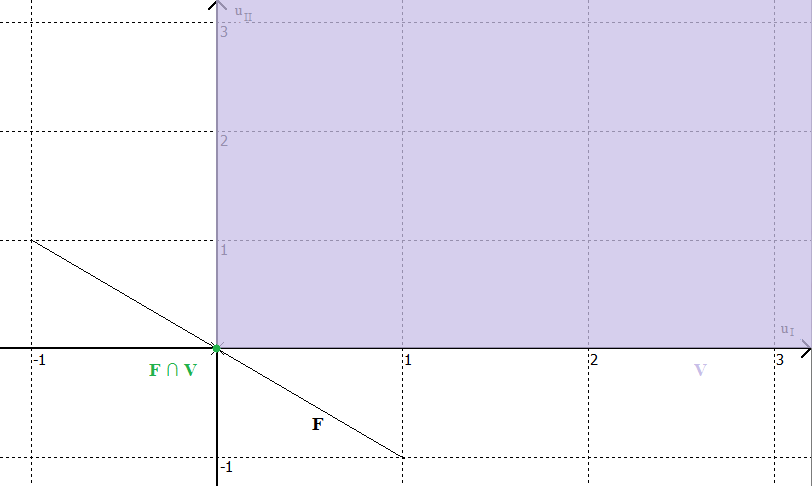
\includegraphics[width=1\textwidth]{graph_2a.png}

\end{document}